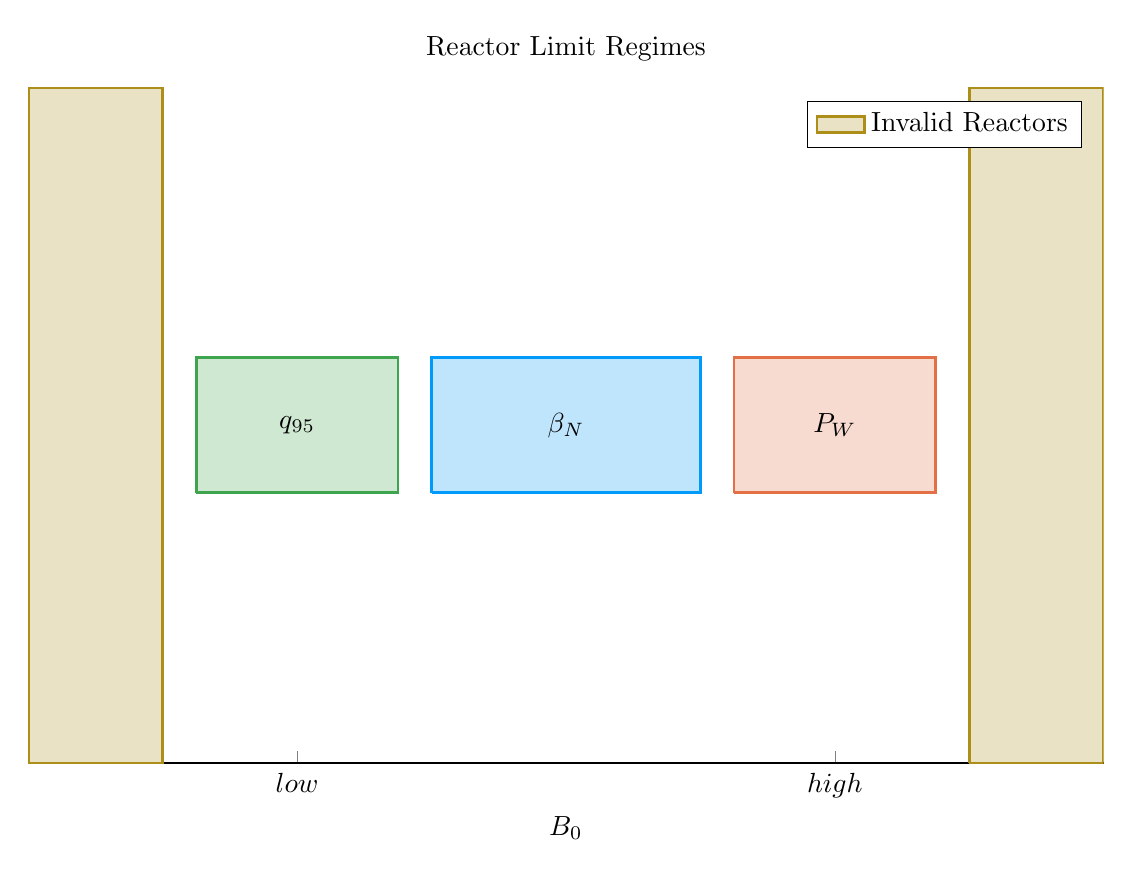
\begin{tikzpicture}[]
\begin{axis}[height = {101.6mm}, ylabel = {}, title = {Reactor Limit Regimes}, xmin = {0.0}, xmax = {8.0}, ymax = {1.0}, xlabel = {$B_0$}, {unbounded coords=jump, scaled x ticks = false, xticklabel style={rotate = 0}, xmajorgrids = false, xtick = {2,6}, xticklabels = {$low$,$high$}, xtick align = inside, axis lines* = left, scaled y ticks = false, yticklabel style={rotate = 0}, ymajorticks=false, ymajorgrids = false, axis lines* = left,     xshift = 0.0mm,
    yshift = 0.0mm,
    axis background/.style={fill={rgb,1:red,1.00000000;green,1.00000000;blue,1.00000000}}
, colorbar style={title=}}, ymin = {0.0}, width = {152.4mm}]\addplot+ [color = {rgb,1:red,0.67554396;green,0.55566233;blue,0.09423434},
draw opacity=1.0,
line width=1,
solid,mark = none,
mark size = 2.0,
mark options = {
    color = {rgb,1:red,0.00000000;green,0.00000000;blue,0.00000000}, draw opacity = 1.0,
    fill = {rgb,1:red,0.67554396;green,0.55566233;blue,0.09423434}, fill opacity = 1.0,
    line width = 1,
    rotate = 0,
    solid
},fill = {rgb,1:red,0.67554396;green,0.55566233;blue,0.09423434}, fill opacity=0.25,area legend]coordinates {
(0, 0)
(1, 0)
(1, 1)
(0, 1)
(0, 0)
};
\addlegendentry{Invalid Reactors}
\addplot+ [color = {rgb,1:red,0.67554396;green,0.55566233;blue,0.09423434},
draw opacity=1.0,
line width=1,
solid,mark = none,
mark size = 2.0,
mark options = {
    color = {rgb,1:red,0.00000000;green,0.00000000;blue,0.00000000}, draw opacity = 1.0,
    fill = {rgb,1:red,0.67554396;green,0.55566233;blue,0.09423434}, fill opacity = 1.0,
    line width = 1,
    rotate = 0,
    solid
},fill = {rgb,1:red,0.67554396;green,0.55566233;blue,0.09423434}, fill opacity=0.25,forget plot]coordinates {
(7, 0)
(8, 0)
(8, 1)
(7, 1)
(7, 0)
};
\addplot+ [color = {rgb,1:red,0.24222430;green,0.64327509;blue,0.30444865},
draw opacity=1.0,
line width=1,
solid,mark = none,
mark size = 2.0,
mark options = {
    color = {rgb,1:red,0.00000000;green,0.00000000;blue,0.00000000}, draw opacity = 1.0,
    fill = {rgb,1:red,0.24222430;green,0.64327509;blue,0.30444865}, fill opacity = 1.0,
    line width = 1,
    rotate = 0,
    solid
},fill = {rgb,1:red,0.24222430;green,0.64327509;blue,0.30444865}, fill opacity=0.25,forget plot]coordinates {
(1.25, 0.4)
(2.75, 0.4)
(2.75, 0.6)
(1.25, 0.6)
(1.25, 0.4)
};
\addplot+ [color = {rgb,1:red,0.00000000;green,0.60560316;blue,0.97868012},
draw opacity=1.0,
line width=1,
solid,mark = none,
mark size = 2.0,
mark options = {
    color = {rgb,1:red,0.00000000;green,0.00000000;blue,0.00000000}, draw opacity = 1.0,
    fill = {rgb,1:red,0.00000000;green,0.60560316;blue,0.97868012}, fill opacity = 1.0,
    line width = 1,
    rotate = 0,
    solid
},fill = {rgb,1:red,0.00000000;green,0.60560316;blue,0.97868012}, fill opacity=0.25,forget plot]coordinates {
(3.0, 0.4)
(5.0, 0.4)
(5.0, 0.6)
(3.0, 0.6)
(3.0, 0.4)
};
\addplot+ [color = {rgb,1:red,0.88887350;green,0.43564919;blue,0.27812294},
draw opacity=1.0,
line width=1,
solid,mark = none,
mark size = 2.0,
mark options = {
    color = {rgb,1:red,0.00000000;green,0.00000000;blue,0.00000000}, draw opacity = 1.0,
    fill = {rgb,1:red,0.88887350;green,0.43564919;blue,0.27812294}, fill opacity = 1.0,
    line width = 1,
    rotate = 0,
    solid
},fill = {rgb,1:red,0.88887350;green,0.43564919;blue,0.27812294}, fill opacity=0.25,forget plot]coordinates {
(5.25, 0.4)
(6.75, 0.4)
(6.75, 0.6)
(5.25, 0.6)
(5.25, 0.4)
};
\node at (axis cs:2, 0.5) [,
color={rgb,1:red,0.00000000;green,0.00000000;blue,0.00000000}, draw opacity=1.0,
rotate=0.0
] {$q_{95}$};
\node at (axis cs:4, 0.5) [,
color={rgb,1:red,0.00000000;green,0.00000000;blue,0.00000000}, draw opacity=1.0,
rotate=0.0
] {$\beta_N$};
\node at (axis cs:6, 0.5) [,
color={rgb,1:red,0.00000000;green,0.00000000;blue,0.00000000}, draw opacity=1.0,
rotate=0.0
] {$P_W$};
\end{axis}

\end{tikzpicture}
